
\chapter{Clustering}
\label{Clustering}

TODO: cluster extension, set detection (specyfying set of individuals using
small set of parameters, e.g center and radius),
we make an assumption that clusters are good apprximation of basins of
attraction,
clustering metrics,
clustering as an effective stop criterion (definition of the stop criterion,
problems)

Clustering is used as a stand-alone tool to get insight into the distribution
of a data set or as a preprocessing step for other algorithms operating on the
detected clusters. The latter usecase is used in our deterioration schema.

We have choosen density-base clustering algorihtm called \textit{OPTICS:
Ordering Points To Identify the Clustering Structure} \cite{optics}. In density
clustering clusters are regarded as regions in the data space in which the objects are 
dense and which are separated by regions of low object density. These regions
may have an arbitrary shape and the points inside a region may be arbitrarily
distributed.

\section{Cluster Extension}

\section{Clustering as a Stop Criterion}

\section{OPTICS}

TODO: general description, optics ordering, extracting clusters, random samples,
clustering, diagrams, reachability plots,
why optics is good for further deterioration (describe in the next chapter)

\textit{OPTICS} is an extendsion to a well-known density clustering algorithm
called \textit{DBSCAN}. The basic idea for \textit{DBSCAN} is that for each
point of a cluster the neighborhood of a given radius $\epsilon$ has to contain
at least a minimum number of points $minPts$.

\textit{OPTICS} works like dbscan but for an infinite number of distance
paramters $\epsilon_i$ which are smaller than a \textit{generating distance}
$\epsilon$. The only difference is that we do not assing cluster memberships.
Instead, we store the \textbf{order} in which the objects are processed (the
main priniple is that we always have to select an object which is
density-reachable with respect to the lowest $\epsilon$ value to guarantee that
clusters with higher density are finished first) and the information which would
be used by \textit{DBSCAN} algorithm to assing cluster memberships. This
information consists of only two values for each object:
\begin{itemize}
  \item core-distance - the core-distance of an object $p$ is simply the
  smallest distance $\epsilon'$ between $p$ and an object in its
  $\epsilon$-neighborhood such that $p$ would be a core object with respect to
  $\epsilon'$ if this neighbor is contained in $N_\epsilon(p)$. Otherwise, the
  core-distance is \textit{UNDEFINED}
  \item reachability-distance - the reachability-distance of an object $p$ with
  respect to another object $o$ is the smallest distance such that $p$ is
  directly density-reachable from $o$ if $o$ is a core object
\end{itemize}

This information is sufficient to extract all density-based clusterings
with respect to any distance $\epsilon'$ which is smaller that the generating
distance $\epsilon$

An advantage of cluster-ordering a data set compared to other clustering methods
is that the ordering which might be visualized by \textit{reachability-plot} of
ordered points is rather insensitive to the input parameters of the method i.e.
the \textit{generating distance} $\epsilon$ and the value for $minPts$. Roughly
speaking, the values have just to be \textit{large} enough to yield a good
result. The concrete values are not crucial because there is a broad range of
possible values for which we always can see the clustering structure of a data
set when looking at the corresponding \textit{reachability-plot}. Figure 3.1
shows the result of \textit{OPTICS} clustering for a sample set of points.
Figure 3.2 shows reachablity plot for various \textit{generating distances} -
$\epsilon$.

\begin{figure}
  \centering
  \fbox{
    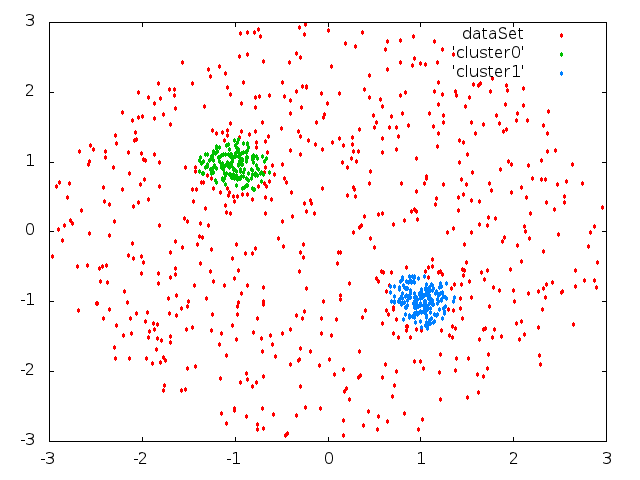
\includegraphics[scale=0.5]{clusters.png}
  }
  \caption{Visualization of the DBSCAN algorithm applied to Optics ordering
  of simple 2-dimensional data set which consists of 1000 points. Optics
  paramters: $minPts=20, \epsilon=1.2$, DBSCAN paramters: $\epsilon'=0.1$ }
  \label{clusters}
\end{figure}


\begin{figure}
  \centering
  \fbox{
    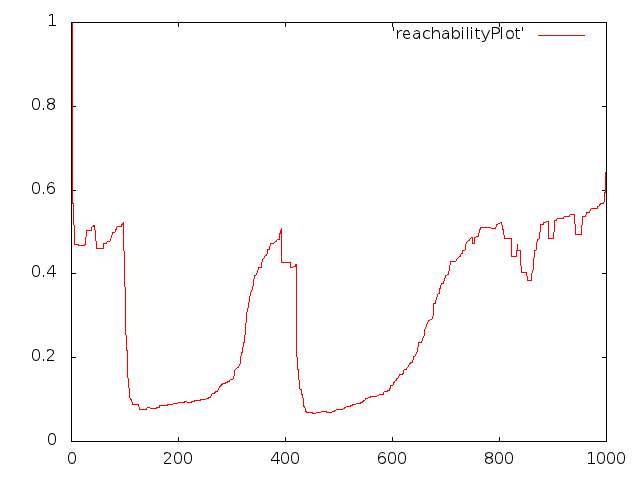
\includegraphics[scale=0.4]{reachability1/1_5_20.png}
  }
  \fbox{
    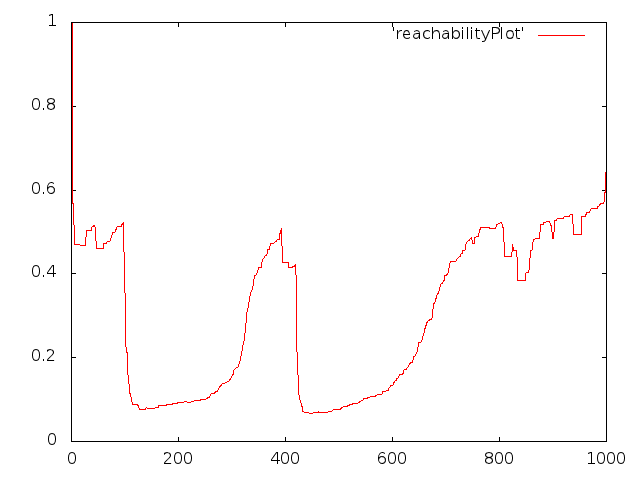
\includegraphics[scale=0.4]{reachability1/1_0_20.png}
  }
  \fbox{
    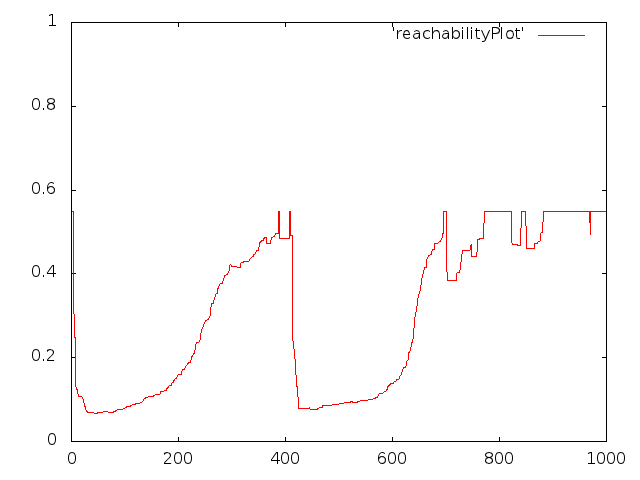
\includegraphics[scale=0.4]{reachability1/0_5_20.png}
  }
  \caption{Reachability plot for data set presented on figure 3.1. Optics
  paramters (minPts, $\epsilon$) are: (20, 1.5), (20, 1.0), (20, 0.5)
  respectively. The two cavities which are visible in each plot depict the two
  of the clusters on figure 3.1. This proves that there is a large range of
  values for $\epsilon$ for which the appearance of the reachability plot will
  not change significantly.}
  \label{reach}
\end{figure}
